\chapter{Application}
\label{chapter:application}


\section{Use cases}
\label{section:useCases}

Before diving into the application architecture and implementation details, let us first describe the use cases to get a complete overview of the functionality the app has to provide (See Fig. \ref{useCase}). The first and the most important use case is registering documents into the system. This would include automatically generating a registration number for each document. It is an important part of automating the current process, in which for registering a new document, the employee has to contact the registry administrator and ask for an available registration number. For the registration to be complete, the user has to specify a destination for the document. In most cases, the document would be internal, meaning that the destination would be other employees of the institution. In this case, the document is sent to the specified recipients, which receive an email notification and could then view the received documents in their account. However, some documents could have an external destination, like another institution or organization. In this case, the destination is specified so the document could be easily tracked in the future. Analogically, the issuer could specify an external source of the document, if it has one.

The user could upload an electronic version of the document, either immediately after the registration, or in any point of time in the future. Additionally, the upload feature is available for all recipients of a document.

The logic behind the document management process relies mainly on two actions: resolving and archiving a document. Basically, when a user receives a document, it means that he or she is expected to perform an action related to it. It could be an action as trivial as aknowledging that the document was received, or something more complex like reading and approving the document, uploading an edited version of the document or sending it further to other users. Regardless of this, the \textbf{resolve} action is meant to finalize the interaction between a user and a document.

\begin{figure}[H]
    \centering
    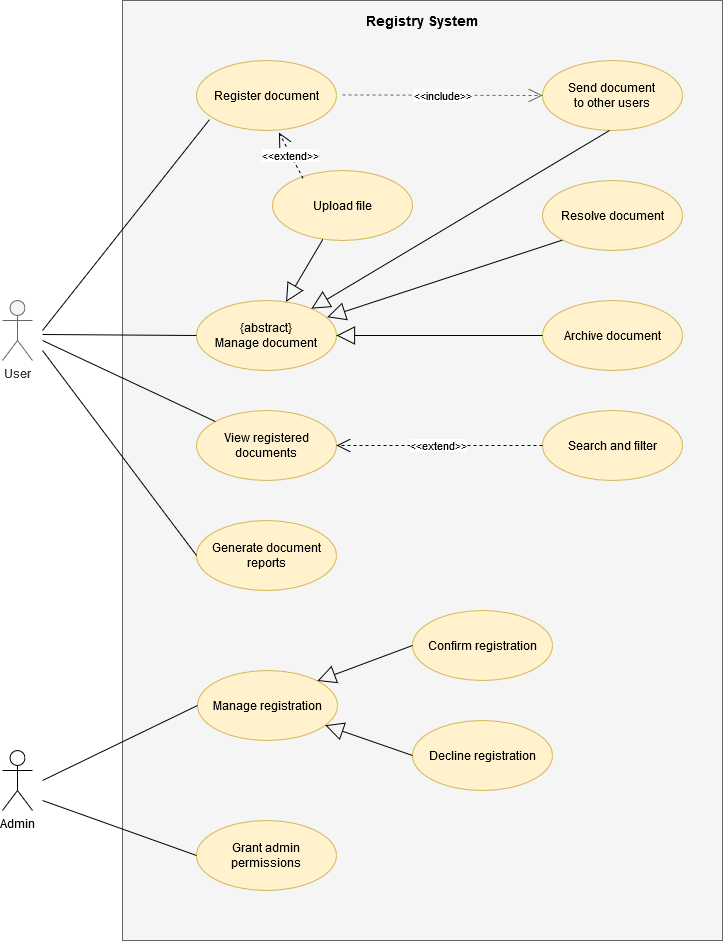
\includegraphics[width=5in]{images/useCase}
    \caption{Registry System Use Cases}
    \label{useCase}
\end{figure}

In simpler terms, marking a document as resolved is telling its issuer that all necessary actions from the receiver were taken.

The \textbf{archive} action, on the other hand, is meant to complete the document lifecycle and can only be performed by the document issuer. After a document is marked as archived, it could no longer get resolved or sent to other users. Resolving and archiving a document are closely related actions. After all, it seems rather logical that the user should only archive a document after it has been resolved by its receiver. However, the logic gets more complicated in case multiple receivers are specified. It could be that all of them have to take different actions on the document. It could also be that getting the document resolved by only one of them would be sufficient, if, for example, they are employees of the same department. In this case, getting a document resolved by a receiver is not a required constraint for the document to get archived. Similarily, when a document is resolved, it does not necessarily imply that it should immediately get archived. That is why we have not constrained the ability to archive a document based on its resolved status, but rather let the issuer do it when he or she deems it necessary. The \textit{Resolve document} and \textit{Archive document} use cases are described in detail in Table \ref{resolveUseCase} and \ref{archiveUseCase}.

\begin{table}[]
    \begin{tabular}{|p{0.3\textwidth}|p{0.6\textwidth}|}
        \hline
        Name                                  & Resolve document                                                  \\ \hline
        Short description                     & A user marks a document as resolved .                             \\ \hline
        Precondition                          & \begin{tabular}[c]{@{}l@{}}The user is logged in to the system.\\ The user is a receiver of the document.\end{tabular}                                         \\ \hline
        Postcondition                         & \begin{tabular}[c]{@{}l@{}}The document shows as resolved by the user in the app.\\ The document issuer receives an email notification.\end{tabular}                                         \\ \hline
        Error situations                      & The server could not perform the operation.                       \\ \hline
        System state in the event of an error & Document is not marked as resolved by the user.                   \\ \hline
        Actors                                & User                                                              \\ \hline
        Trigger                               & All document related actions needed from the user were performed. \\ \hline
        Standard process                      & \begin{tabular}[c]{@{}l@{}}(1) User selects the document.\\ (2) User introduces a resolve message (optional).\\ (3) User confirms the resolve action.\end{tabular}                                         \\ \hline
        Alternative process                   & (3') User cancels the resolve action.                             \\ \hline
    \end{tabular}
    \caption{Use case description for \textit{Resolve document}}
    \label{resolveUseCase}
\end{table}

\begin{table}[H]
    \begin{tabular}{|p{0.3\textwidth}|p{0.6\textwidth}|}
        \hline
        Name                                  & Archive document                                                                     \\ \hline
        Short description                     & A user marks a document as archived.                                                 \\ \hline
        Precondition                          & \begin{tabular}[c]{@{}l@{}}The user is logged in to the system.\\ The user is the issuer of the document.\end{tabular}                                                            \\ \hline
        Postcondition                         & \begin{tabular}[c]{@{}l@{}}The document shows as archived in the app.\\ The document cannot be send to other users or resolved.\end{tabular}                                                            \\ \hline
        Error situations                      & The server could not perform the operation.                                          \\ \hline
        System state in the event of an error & Document is not marked as archived by the user.                                      \\ \hline
        Actors                                & User                                                                                 \\ \hline
        Trigger                               & The document issuer considers that all actions related to the document are complete. \\ \hline
        Standard process                      & \begin{tabular}[c]{@{}l@{}}(1) User selects the document.\\ (2) User introduces an archiving message (optional).\\ (3) User confirms the archive action.\end{tabular}                                                            \\ \hline
        Alternative process                   & (3') User cancels the archive action.                                                \\ \hline
    \end{tabular}
    \caption{Use case description for \textit{Archive document}}
    \label{archiveUseCase}
\end{table}

Aside from managing owned and received documents, users should also have access to the entire register containing all documents cataloged into the sistem. This should include the ability to search for a specific document or filter the list based on different criteria. Another important feature would be generating a report in PDF or XLS that would either include all documents or only a certain subset matching the criteria specified by the user. The reports could then be printed and physically archived in the institution and should therefore replace the register that is currently filled out by hand.

Having a separate account for each user would imply the necessity of a registration process. As it is an internal app, a flow in which the user provides credentials and the account gets automatically created would not be sufficient. We have to also verify that the person requesting the account is an employee of the institution to which the application belongs. To achieve this, we would add the \textbf{Admin} role to our system. Admins would inherit all document management rights that the simple users have, but will also have special permissions that would allow them to manage the registration of new users.

\begin{figure}[H]
    \centering
    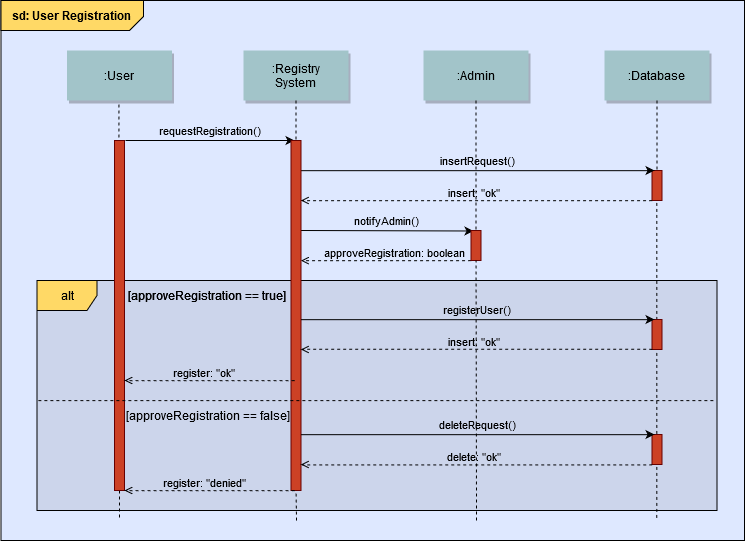
\includegraphics[width=5in]{images/sequenceDiagram}
    \caption{Sequence diagram for the \textit{User Registration} flow}
    \label{sequenceDiagram}
\end{figure}

As seen in Fig. \ref{sequenceDiagram}, the registration process begins with a user sending a request to the system to register a new account. The system then inserts the request into the database and sends an email notification to each of the Admins telling them that a new registration has been requested. The admins could then either confirm or decline the registration. In case of confirmation, the registration is completed within the database and the user is notified that the registration was successful. He or she can from that moment access the newly created account using the login credentials provided at the time of registration. In case an admin denies the registration, all information about the user is deleted from the database and a notification is sent to inform the user that his request was denied.



\section{Architecture}
\label{section:architecture}



\section{Implementation}
\label{section:implementation}


